%%%%%%%%%%%%%%%%%%%%%%%%%%%%%%%%%
%
%       EXERCÍCIO
%
%%%%%%%%%%%%%%%%%%%%%%%%%%%%%%%%%

\definevalorquestao

\begin{exercicioBanco}[\valorquestao]
O valor de um equipamento industrial sofre depreciação com o passar dos anos de acordo com o gráfico a seguir, que cobre um período de \(4\) anos.

\begin{center}
    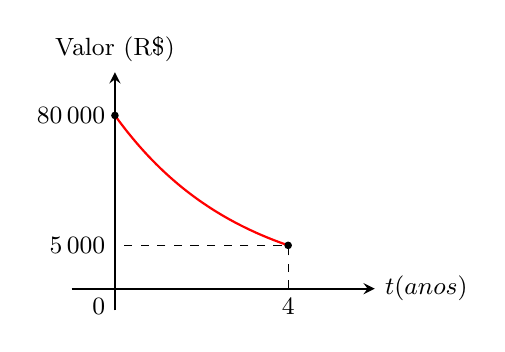
\begin{tikzpicture}[scale=0.55, >=stealth]
        % Eixos
        \draw[->, thick] (-1,0) -- (6,0) node[right] {\small $t \text{ (anos)}$};
        \draw[->, thick] (0,-0.5) -- (0,5) node[above] {\small Valor (R\$)};
        
        % Linhas pontilhadas
        \draw[dashed] (4,0) -- (4,1) -- (0,1);
        
        % Pontos e marcações
        \node[left] at (0,4) {\small \(80\,000\)};
        \node[left] at (0,1) {\small \(5\,000\)};
        \node[below left] at (0,0) {\small \(0\)};
        \node[below] at (4,0) {\small \(4\)};

        % Curva exponencial f(t) = 4 * (1/2)^t
        % Em t=0: 4*(0.5)^0 = 4
        % Em t=4: 4*(0.5)^2 não, para passar em (4,1): 4 * (0.5)^(\x/2)
        \draw[domain=0:4, smooth, samples=100, thick, red] 
            plot (\x, {4*(0.5)^(\x/2)});

        \fill (0,4) circle (2.5pt);
        \fill (4,1) circle (2.5pt);
    \end{tikzpicture}
\end{center}

Sabendo que o valor do equipamento em função do tempo é modelado por \(V(t) = k \cdot a^t\), determine os valores reais das constantes \(k\) e \(a\).

\newcommand{\alternativas}{%
    \begin{center}
        \begin{tabularx}{\textwidth}{XXX}
            (a) \(k = 80\,000\) e \(a = \dfrac{1}{4}\). &
            (b) \(k = 80\,000\) e \(a = \dfrac{1}{2}\). &
            (c) \(k = 5\,000\) e \(a = 2\). \\[15pt]
            (d) \(k = 40\,000\) e \(a = \dfrac{1}{16}\). &
            (e) \(k = 80\,000\) e \(a = \dfrac{1}{8}\).
        \end{tabularx}
    \end{center}
}

\newcommand{\resposta}{B}

% Lógica condicional para exibição
\ifdefstring{\atividade}{lista}{%
    \alternativas
    \vspace{0.5em}
    
    \noindent\textbf{Resposta:} letra \textbf{\resposta}.
}{%
    \ifdefstring{\modo}{objetivo}{%
        \alternativas
    }{%
        % modo = discursiva → não mostra alternativas
    }
}
\end{exercicioBanco}

